\documentclass[14pt]{beamer}
\title{WEB :: JavaScript}
\author[TS]{TalentSprint}
\institute[L\&D]{Licensed To Skill}
\usefonttheme{serif}
\usepackage{fancybox}
\usecolortheme{orchid}
\usepackage{bookman}
\usepackage{multirow}
\usepackage{hyperref}
\usepackage[T1]{fontenc}
\usepackage{graphicx}
\usepackage{listings}
\graphicspath{{../Images/}}
\usepackage[tikz]{bclogo}
\usepackage{soul}
\usepackage{array}
 \definecolor{light-gray}{gray}{0.80}
 \usepackage{color}
\beamertemplateballitem
\usebackgroundtemplate{
\includegraphics[width=\paperwidth]{TS-XP-Logo.jpg}}
\lstset{language=html, numbers=left, numbers=none, basicstyle=\footnotesize, numberstyle=\tiny,  numbersep=10pt, showstringspaces=false, breaklines=true,keepspaces=true, columns=flexible}
\begin{document}

\begin{frame}
  \titlepage
\end{frame}

\begin{frame}{Learning Objectives}
The content in this presentation is aimed at teaching  learners to:
  \begin{itemize}
  \item Work on regular expressions
  \item Validate HTML WebPages
  \end{itemize}
\end{frame}

\begin{frame}{Java Script}
\textbf{Form Validation}
\begin{itemize}
 \item Used to occur at the server, after the client had entered all necessary data and then pressed the Submit button.
 \item The server would have to send all the data back to the client and request that the form be resubmitted with correct information. 
\end{itemize}
\end{frame}

\begin{frame}{JavaScript}
\textbf{Form Validation}
\begin{itemize}
 \item This was really a lengthy process and over burdening server. 
 \item JavaScript provides a way to validate form's data on the client's computer.
\end{itemize}
\end{frame}

\begin{frame}{JavaScript}
\textbf{Form Validation Functions}

\vspace{1pc}
Basic Validation:
\begin{itemize}
 \item Make sure that data was entered into each form field that required it.
 \item We will call validate() function to validate data when onsubmit event is occurring.
\end{itemize}
\end{frame}

\begin{frame}{JavaScript}
\textbf{Form Validation Functions}

\vspace{1pc}
Data Format Validation:
\begin{itemize}
 \item Entered data must be checked for correct form and value.
 \item We can RegExp for validation of data.
\end{itemize}
\end{frame}

\begin{frame}{JavaScript}
\textbf{Regular Expressions and RegExp Object}
\begin{itemize}
 \item An object that describes a pattern of characters.
 \item The JavaScript RegExp class represents regular expressions, and both String and RegExp define methods that use regular expressions to perform powerful pattern-matching and search and replace functions on text.
\end{itemize}
\end{frame}

\begin{frame}{JavaScript}
\textbf{Regular Expressions and RegExp Object}
\begin{itemize}
 \item A regular expression could be defined with the RegExp() constructor:
 \begin{block}{}
  \lstinline!var pattern = new RegExp(pattern, attributes);!
  
  \lstinline!var pattern = /pattern/attributes;!
 \end{block}
\end{itemize}
\end{frame}

\begin{frame}{JavaScript}
Browsers Compatibility
\begin{itemize}
 \item Understand the differences between different browsers in order to handle each in the way it is expected.
 \item To get information about the browser your Web page is currently running in, use the built-in navigator object.
\end{itemize}
\end{frame}

\begin{frame}{JavaScript}
Validation
\begin{figure}[H]
 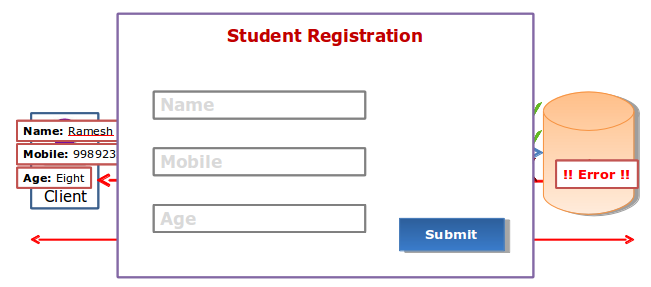
\includegraphics[scale=.4]{validation.png}
\end{figure}
\end{frame}

\begin{frame}{JavaScript}
Validation
\begin{figure}[H]
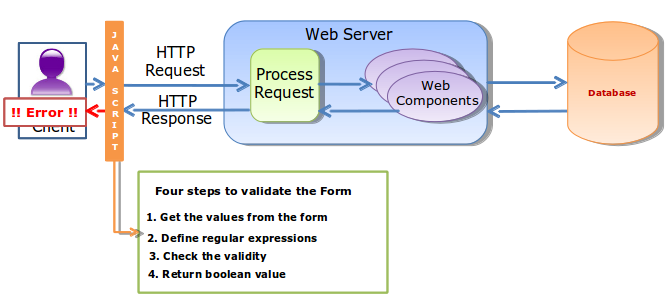
\includegraphics[scale=.45]{steps-to-validate.png}
\end{figure}
\end{frame}

\begin{frame}{JavaScript}
Validation
\begin{block}{}
\lstinline! <form name = ``reg'' action = ``TargetServer'' onsubmit = ``return validate()''>!
\end{block}
if \textbf{validate()}
\begin{itemize}
 \item returns TRUE form will be submitted
 \item returns FALSE form will NOT be submitted
\end{itemize}
\end{frame}

\begin{frame}{JavaScript}
\textcolor{red}{Student Registration}

\vspace{1pc}
\framebox[4cm][l]{\color{light-gray}Name}
\begin{block}{}
\lstinline!<input type = ``text'' placeholder = ``Name'' name = ``!\colorbox{orange}{sname}!''>!
\end{block} 
Should accept only alphanumeric characters, dot and space Minimum 6 and Maximum 20 characters
\end{frame}

\begin{frame}{JavaScript}
\framebox[4cm][l]{\color{light-gray}Mobile}
\begin{block}{}
\lstinline!<input type = ``text'' placeholder = ``Mobile'' name = ``!\colorbox{orange}{mob}!''>!
\end{block} 
Should accept exactly 0 digits (0-9), Should starts with 9 or 8 or 7
\end{frame}

\begin{frame}{JavaScript}
\framebox[4cm][l]{\color{light-gray}Age}
\begin{block}{}
\lstinline!<input type = ``text'' placeholder = ``Age'' name = ``!\colorbox{orange}{age}!''>!
\end{block} 
Should accept only max 2 digits (0-9)
\begin{block}{}
\colorbox{orange}{Submit}

\lstinline!</form>!
\end{block}
\end{frame}

\begin{frame}[fragile]{JavaScript}
Validation
\begin{description}
 \item [Step - 1] Get the Value of text fields
\end{description}
\begin{block}{Syntax}
\begin{lstlisting}
var value = document.<form_name>.<field_name>.value
    or
var value = document.getElementById(``element_id'').value
\end{lstlisting}
\end{block}
\begin{block}{Snippet}
\begin{lstlisting}
var name = document.reg.sname.value;
var mob = document.reg.mob.value;
var age = document.reg.age.value;
\end{lstlisting}
\end{block}
\end{frame}

\begin{frame}[fragile]{JavaScript}
\begin{description}
 \item [Step - 2] Define Regular Expression
\end{description}
\begin{block}{Syntax}
 \lstinline!var exp = new RegExp(``pattern'');!
\end{block}
\begin{block}{Snippet}
\begin{lstlisting}
var rname = new RegExp(``^[a-zA-Z .]{6,10}$'');
var rmob = new RegExp(``^[987][0-9]{9}$'');
var rage = new RegExp(``^[0-9]{1,2}$'');
\end{lstlisting}
\end{block}
\end{frame}

\begin{frame}{JavaScript}
Brackets
\begin{description}
 \item [$\lbrack$...$\rbrack$] Any one character between the brackets.
 \item [$\lbrack$ $\wedge$...$\rbrack$] Any one character not between the brackets.
 \item [$\lbrack$0-9$\rbrack$] It matches any decimal digit from 0 through 9.
\end{description}
\end{frame}

\begin{frame}{JavaScript}
Brackets
\begin{description}
 \item [$\lbrack$a-z$\rbrack$] It matches any character from lowercase a through lowercase z.
 \item [$\lbrack$A-Z$\rbrack$] It matches any character from uppercase A through uppercase Z.
 \item [$\lbrack$a-Z$\rbrack$] It matches any character from lowercase a through uppercase Z.
\end{description}
\end{frame}

\begin{frame}{JavaScript}
Quantifiers
\begin{description}
 \item [p+] It matches any string containing at least one p.
 \item [p*] It matches any string containing zero or more p's.
 \item [p?] It matches any string containing one or more p's.
 \item [p{N}] It matches any string containing a sequence of N p's.
\end{description}
\end{frame}

\begin{frame}{JavaScript}
Quantifiers
\begin{description}
 \item [p{2,3}] It matches any string containing a sequence of two or three p's.
 \item [p{2, }] It matches any string containing a sequence of at least two p's.
 \item [p\$] It matches any string with p at the end of it.
 \item [$\wedge$p] It matches any string with p at the beginning of it.
\end{description}
\end{frame}

\begin{frame}{JavaScript}
Metacharacters
\begin{description}
 \item [.] a single character
 \item [$\backslash$s] a whitespace character (space, tab, newline)
 \item [$\backslash$S] non-whitespace character
 \item [$\backslash$d] a digit (0-9)
 \item [$\backslash$D] a non-digit
 \item [$\backslash$w] a word character (a-z, A-Z, 0-9, \_)
\end{description}
\end{frame}

\begin{frame}{JavaScript}
Metacharacters
\begin{description}
 \item [$\backslash$W] a non-word character
 \item [$\lbrack$$\backslash$b$\rbrack$] a literal backspace (special case)
 \item [$\lbrack$aeiou$\rbrack$] matches a single character in the given set
 \item [$\lbrack$$\wedge$aeiou$\rbrack$] matches a single character outside the given set
\end{description}
\end{frame}

\begin{frame}[fragile]{JavaScript}
\begin{description}
 \item [Step - 3] Check the validity
\end{description}
\textbf{Syntax:} \lstinline!regexp.test(data)!
\begin{block}{Snippet}
\begin{lstlisting}
if (rname.test(name))
    if (rmob.test(mob))
        if (rage.mob(age))
            return true;
        else
            return false;
    else
        return false;
else
    return false;
\end{lstlisting}
\end{block}
\end{frame}

\begin{frame}{JavaScript}
\begin{description}
 \item [Step - 4] Return boolean value
\end{description}
\end{frame}

\begin{frame}{JavaScript}
RegExp Methods
\begin{description}
 \item [exec()] executes a search for a match in its string parameter.
 \item [test()] tests for a match in its string parameter.
 \item [toSource()] returns an object literal representing the specified object; you can use this value to create a new object.
 \item [toString()] returns a string representing the specified object.
\end{description}
\end{frame}

\begin{frame}[fragile]{JavaScript}
\begin{block}{Complete Program}
\begin{lstlisting}
function validate(){
    var name = document.reg.sname.value;
    var mob = document.reg.mob.value;
    var age = document.reg.age.value;
    var rname = new RegExp("^[a-zA-Z .]{6,10}$");
    var rmob = new RegExp("^[987][0-9]{9}$");
    var rage = new RegExp("^[0-9]{1,2}$");
\end{lstlisting}
\end{block}
\end{frame}

\begin{frame}[fragile]{JavaScript}
\begin{block}{Complete Program - Cont...}
\begin{lstlisting}
    if(rname.test(name))
        if(rmob.test(mob))
            if(rage.mob(age))
                return true;
            else
                return false;
        else
            return false;
    else
        return false;
}
\end{lstlisting}
\end{block}
\end{frame}

\begin{frame}{JavaScript}
 \begin{figure}[H]
    
\includegraphics[scale=.3]{qa.png}   
   \end{figure}
\end{frame}

\end{document}
